\documentclass[10pt]{article}
\usepackage[paperwidth=4.25in, paperheight=5.5in, top=0.25in, left=0.5in, right=0.25in, bottom=0.25in]{geometry}
\usepackage{graphicx}

\usepackage[light]{antpolt}
\usepackage[T1]{fontenc}


\usepackage[none]{hyphenat}

\usepackage[utf8]{inputenc}

\begin{document}
\pagestyle{empty}

\centering{
  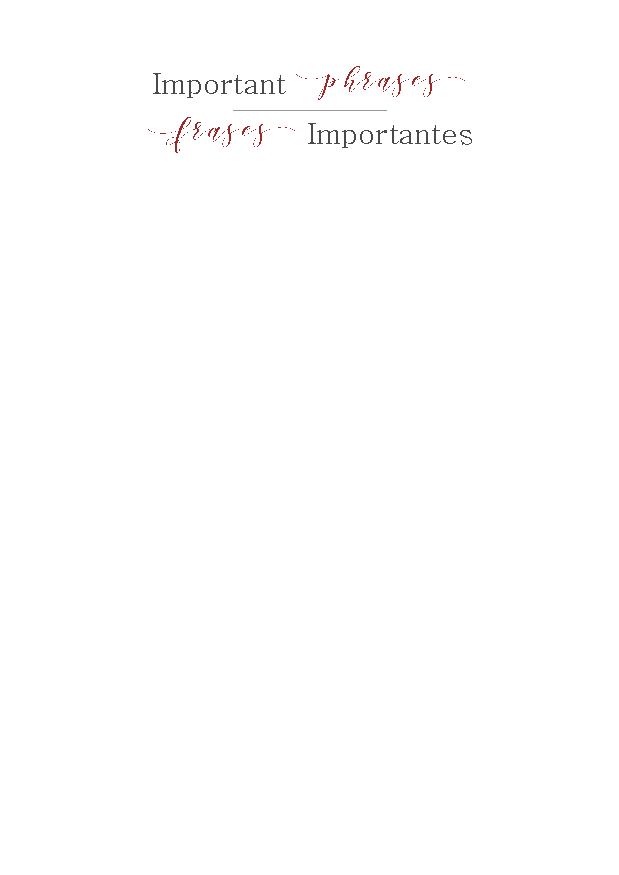
\includegraphics[height=0.75in]{img/important_phrases}
}

\begin{tabular}{p{1.5in}|p{1.5in}}
  The bride and groom are very beautiful!
  &
  Os noivos são muito bonitos!
  \vspace{0.1in}
  \\
  The wedding will be May 20, 2017.
  &
  O casamento será no dia 20 de Maio, 2017
  \vspace{0.1in}
  \\
  I know the bride! I know the groom! 
  &
  Eu conheço a noiva! Eu conheço o noivo!
  \vspace{0.1in}
  \\
  Where is the bathroom?
  &
  Onde é a casa de banho?
  \vspace{0.1in}
  \\
  Thank you.
  &
  Obrigado (if you are a man). Obrigada (if you are a woman).
  \vspace{0.1in}
  \\
  I would like a glass of...
  &
  Eu quero um copo de...
  \vspace{0.1in}
  \\
  \hspace{0.1in}...water & \hspace{0.1in}...água\\
  \hspace{0.1in}...wine & \hspace{0.1in}...vinho\\
  \hspace{0.1in}...juice & \hspace{0.1in}...sumo\\
  \vspace{0.1in}
  \\
  Do you have a website? & Têm uma página na Internet?\\
  {\scriptsize http://www.rubenandjustine.com} & {\scriptsize http://www.rubenandjustine.com}\\
\end{tabular}
\vspace{1in}

\end{document}
